\section{Batch mean loss used in the experiments}\label{appendix:batch_mean}
\textbf{All experiments use a mean over valid tokens within each response, followed by a mean over responses in the batch.} This section specifies the reduction independently of advantage normalization.

Let $m_{i,t}\in\{0,1\}$ indicate a valid response token included in the policy loss, and let $n_i=\sum_t m_{i,t}>0$. For $B$ responses, the policy loss is
\begin{equation}
 \boxed{
 L_{\mathrm{PG}}(\theta)=\frac{1}{B}\sum_{i=1}^{B}
 \left[\frac{1}{n_i}\sum_t m_{i,t}\,\ell_{i,t}(\theta)\right],
 \qquad
 \ell_{i,t}(\theta)=-f_{i,t}(\theta,\sg[\widehat A_{i,t}]).
 }
 \label{eq:batch_mean}
\end{equation}
Here $f$ is the clipped surrogate in \cref{eq:clipped}, and $\sg$ denotes stop-gradient. Padding and positions outside the response loss mask do not enter the numerator or token count. The separate $k_2$ term in \cref{eq:baseline_loss} uses the same reduction.

\paragraph{Response weighting.}
Each response has outer weight $1/B$, and each valid token within response $i$ has weight $1/(Bn_i)$. This differs from dividing the sum of all token losses by the total number of valid tokens:
\begin{equation}
 L_{\mathrm{token}}=\frac{\sum_{i,t}m_{i,t}\ell_{i,t}}{\sum_i n_i}.
\end{equation}
The latter weights each response in proportion to its length. The two reductions agree when all responses have equal length. With a fixed number $k$ of responses per prompt, batch averaging is also equivalent to averaging the per-response losses within each prompt and then across prompts.

\paragraph{Minibatches and accumulation.}
For a minibatch $\mathcal M$, replace $B$ by $|\mathcal M|$ in \cref{eq:batch_mean}. To recover the same mean when combining uneven microbatches or distributed shards, their loss sums must be weighted by their response counts. The normalization moments are associated with the rollout batch; changing the partition into minibatches does not change the definition of the already computed advantages.

\paragraph{Terminal reward and token returns.}
For the basic variant, the immediate reward can be written as
\begin{equation}
 \widetilde r_{i,t}=\mathbf{1}\{t=T_i\}r(q_i,o_i)-\beta d_{i,t}.
\end{equation}
With unit discount, its return is $\sum_{u=t}^{T_i}\widetilde r_{i,u}=G_{i,t}$ from \cref{eq:return}. Thus, a terminal task reward contributes to the return at every preceding response position. For \baseline, the group-centered terminal reward in \cref{eq:group_center} is broadcast to response positions before global normalization.

\clearpage
\section{Finite-sample properties of normalization}\label{appendix:normalization}
We analyze a scalar model to make the effect of estimating normalization statistics from the same samples explicit. Let
\begin{equation}
 r_i=\mu+\epsilon_i,\qquad \epsilon_i\overset{\mathrm{i.i.d.}}{\sim}\mathcal N(0,\sigma^2),\qquad \sigma>0,
\end{equation}
and define $\bar\epsilon=N^{-1}\sum_i\epsilon_i$,
$D_N^2=N^{-1}\sum_i(\epsilon_i-\bar\epsilon)^2$, and
$Z_{i,N}=(\epsilon_i-\bar\epsilon)/D_N$ for $N\geq2$. The population-standardized target is $\epsilon_i/\sigma$. We omit the numerical stabilizer for this analysis; $D_N>0$ almost surely under the stated model.

\begin{proposition}[Finite-sample bound]\label{prop:bound}
For any nonconstant sample of size $N\geq2$, $|Z_{i,N}|\leq\sqrt{N-1}$.
Consequently, under the Gaussian model, $\E[Z_{i,N}\mid\epsilon_i]$ cannot equal $\epsilon_i/\sigma$ almost surely for finite $N$.
\end{proposition}
\begin{proof}
Set $x_j=\epsilon_j-\bar\epsilon$, so $\sum_jx_j=0$. By Cauchy--Schwarz,
\begin{equation}
 x_i^2=\left(\sum_{j\ne i}x_j\right)^2
 \leq(N-1)\sum_{j\ne i}x_j^2.
\end{equation}
Therefore $\sum_jx_j^2\geq Nx_i^2/(N-1)$, giving
$Z_{i,N}^2=Nx_i^2/\sum_jx_j^2\leq N-1$.
The conditional expectation obeys the same bound, whereas
$|\epsilon_i|/\sigma>\sqrt{N-1}$ has positive probability for a Gaussian variable. Equality with the standardized target cannot hold almost surely.
\end{proof}

\paragraph{An exact two-response example.}
For $N=2$, $D_2=|\epsilon_1-\epsilon_2|/2$ and
$Z_{1,2}=\operatorname{sign}(\epsilon_1-\epsilon_2)$ almost surely. Thus,
\begin{equation}
 \E[Z_{1,2}\mid\epsilon_1=x]=2\Phi(x/\sigma)-1,
 \label{eq:two_sample}
\end{equation}
where $\Phi$ is the standard normal cumulative distribution function. This bounded, nonlinear function differs from the linear population-standardized value $x/\sigma$. It illustrates how a small group changes the reward scale through self-normalization.

\begin{proposition}[Large-sample limit]\label{prop:limit}
Under the Gaussian model, for any fixed $i$, $Z_{i,N}\to\epsilon_i/\sigma$ almost surely and in $L^1$ as $N\to\infty$. In particular,
\begin{equation}
 \E\left[\left|\E[Z_{i,N}\mid\epsilon_i]-\epsilon_i/\sigma\right|\right]\longrightarrow0.
\end{equation}
\end{proposition}
\begin{proof}
The strong law gives $\bar\epsilon\to0$ and $D_N^2\to\sigma^2$ almost surely, establishing the first limit. By exchangeability and $\sum_{j=1}^{N}Z_{j,N}^2=N$, we have $\E[Z_{i,N}^2]=1$ for every $N$. This uniform second-moment bound implies uniform integrability, so the almost-sure convergence also holds in $L^1$. Conditional Jensen's inequality gives
\begin{equation}
 \E\left[\left|\E[Z_{i,N}-\epsilon_i/\sigma\mid\epsilon_i]\right|\right]
 \leq\E\left[|Z_{i,N}-\epsilon_i/\sigma|\right]\to0.
\end{equation}
\end{proof}

\paragraph{Implications for global normalization.}
The propositions isolate the effect of normalization sample size: estimated moments approach their population values as the number of independent observations grows. A shared batch scale can use observations across many prompt groups, rather than estimating a separate scale from each small group. For grouped or token-level data, the interpretation depends on the number of independently sampled trajectories and their dependence structure.

\paragraph{Relationship to baselines and gradients.}
For an unscaled group mean, $\E[r_i-\bar r_q\mid r_i,q]=(1-1/k)(r_i-\mu_q)$ when responses are conditionally independent with mean reward $\mu_q$. This is the same factor appearing in \cref{eq:rloo_relation}. The propositions concern convergence to a standardized scalar target, distinct from unbiasedness of a policy-gradient estimator. Their role is to explain the normalization mechanism under explicit sampling assumptions.

\clearpage
\section{KL regularization as a gradient surrogate}\label{appendix:kl}
For a fixed context, write $p_\theta(y)=\pi_\theta(y\mid h)$, $q(y)=\pi_{\mathrm{ref}}(y\mid h)$, and $z(y)=\log[p_\theta(y)/q(y)]$. Assume common support and sufficient regularity to interchange differentiation and expectation. The reverse KL is
\begin{equation}
 \KL(p_\theta\|q)=\E_{y\sim p_\theta}[z(y)],
 \qquad
 \nabla_\theta\KL(p_\theta\|q)
 =\E_{p_\theta}[z(y)\nabla_\theta\log p_\theta(y)],
 \label{eq:rkl_gradient}
\end{equation}
using $\E_{p_\theta}[\nabla_\theta\log p_\theta]=0$.

\paragraph{Value estimators and differentiated losses.}
The common expressions are
\begin{equation}
 k_1(z)=z,\qquad k_2(z)=\tfrac12 z^2,\qquad k_3(z)=e^{-z}-1+z.
\end{equation}
Both $k_1$ and $k_3$ have expectation $\KL(p_\theta\|q)$ under on-policy sampling, since $\E_{p_\theta}[e^{-z}]=1$. When sampled actions are treated as fixed during automatic differentiation, their pointwise gradients differ:
\begin{equation}
\begin{aligned}
 \nabla_\theta k_1 &=\nabla_\theta\log p_\theta,\\
 \nabla_\theta k_2 &=z\nabla_\theta\log p_\theta,\\
 \nabla_\theta k_3 &=(1-q/p_\theta)\nabla_\theta\log p_\theta.
\end{aligned}
\label{eq:kl_pointwise}
\end{equation}
The on-policy expectation of the $k_2$ pointwise gradient is exactly \cref{eq:rkl_gradient}. This is the gradient-surrogate interpretation used for the separate KL term in \baseline~\citep{liu2025rethinking}. It is distinct from differentiating the entire expectation $\E_{p_\theta}[k_2]$, which also differentiates the sampling distribution.

Under the same fixed-context assumptions, the expected pointwise gradient of $k_1$ is zero. The $k_1$ expression can instead enter the reward and act as a detached score-function coefficient, as in the returns used by the basic variant. The expected pointwise gradient of $k_3$ equals $-\E_q[\nabla_\theta\log p_\theta]$, the forward-KL gradient. Its value-estimation and loss-gradient roles should therefore be distinguished.

\paragraph{Rollout reuse.}
The on-policy identities apply when the sampled actions follow the current policy. For actions sampled from $p_{\mathrm{old}}$, a fixed-context importance-weighted gradient satisfies
\begin{equation}
 \E_{p_{\mathrm{old}}}\left[
 \frac{p_\theta(y)}{p_{\mathrm{old}}(y)}z(y)\nabla_\theta\log p_\theta(y)
 \right]=\nabla_\theta\KL(p_\theta\|q).
\end{equation}
The practical separate loss in \cref{eq:baseline_loss} is the unweighted $k_2$ surrogate on the rollout data. Its exact gradient-equivalence interpretation applies at the on-policy point; subsequent optimization uses it as a surrogate. For autoregressive policies, the fixed-context statement concerns the conditional next-token distribution.

\clearpage
\section{Additional training traces}\label{appendix:curves}
\begin{figure}[h!]
\centering
\begin{subfigure}{0.93\linewidth}
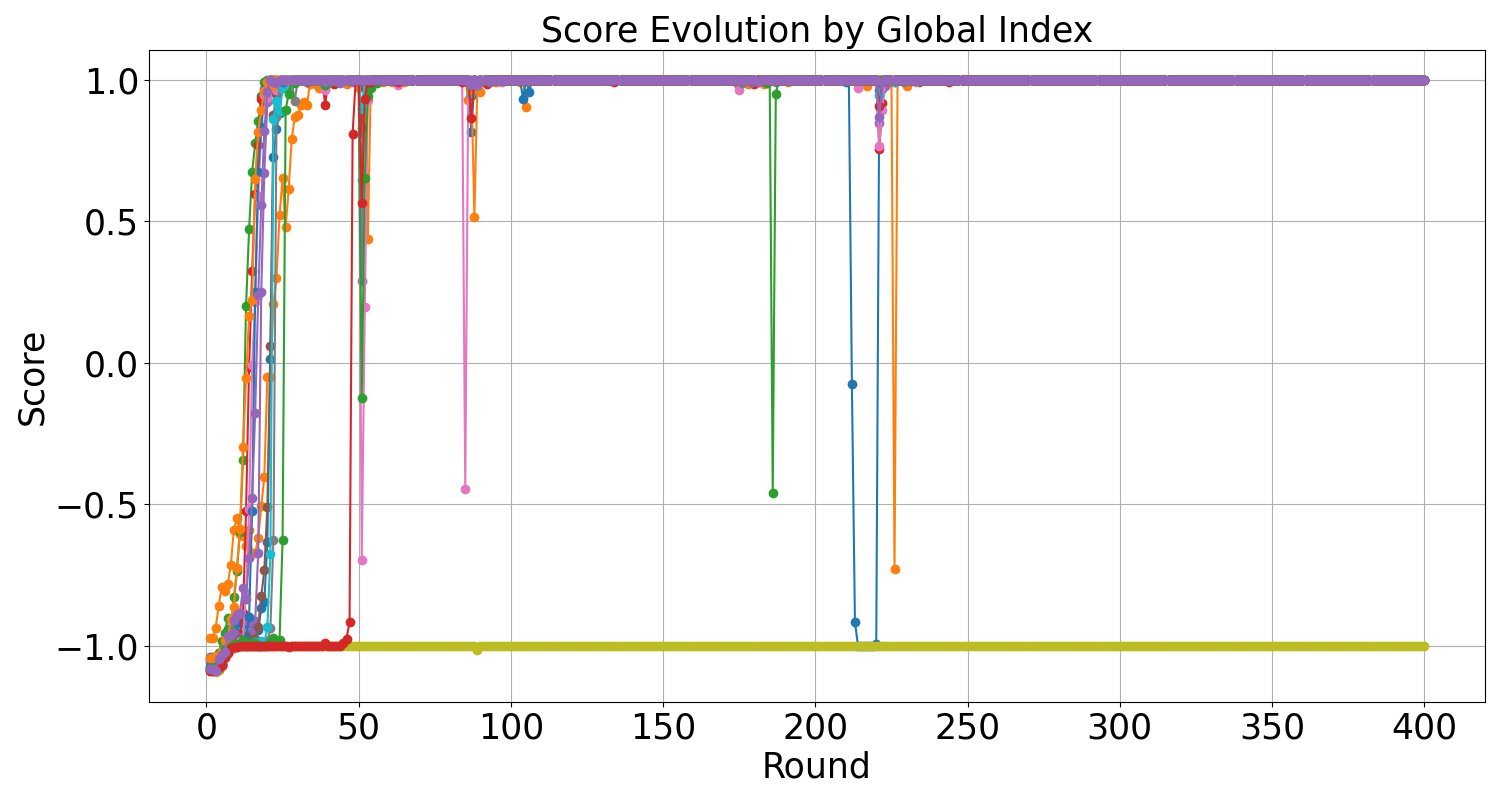
\includegraphics[width=\linewidth]{imgs/GRPO.png}
\caption{GRPO}
\end{subfigure}

\medskip
\begin{subfigure}{0.93\linewidth}
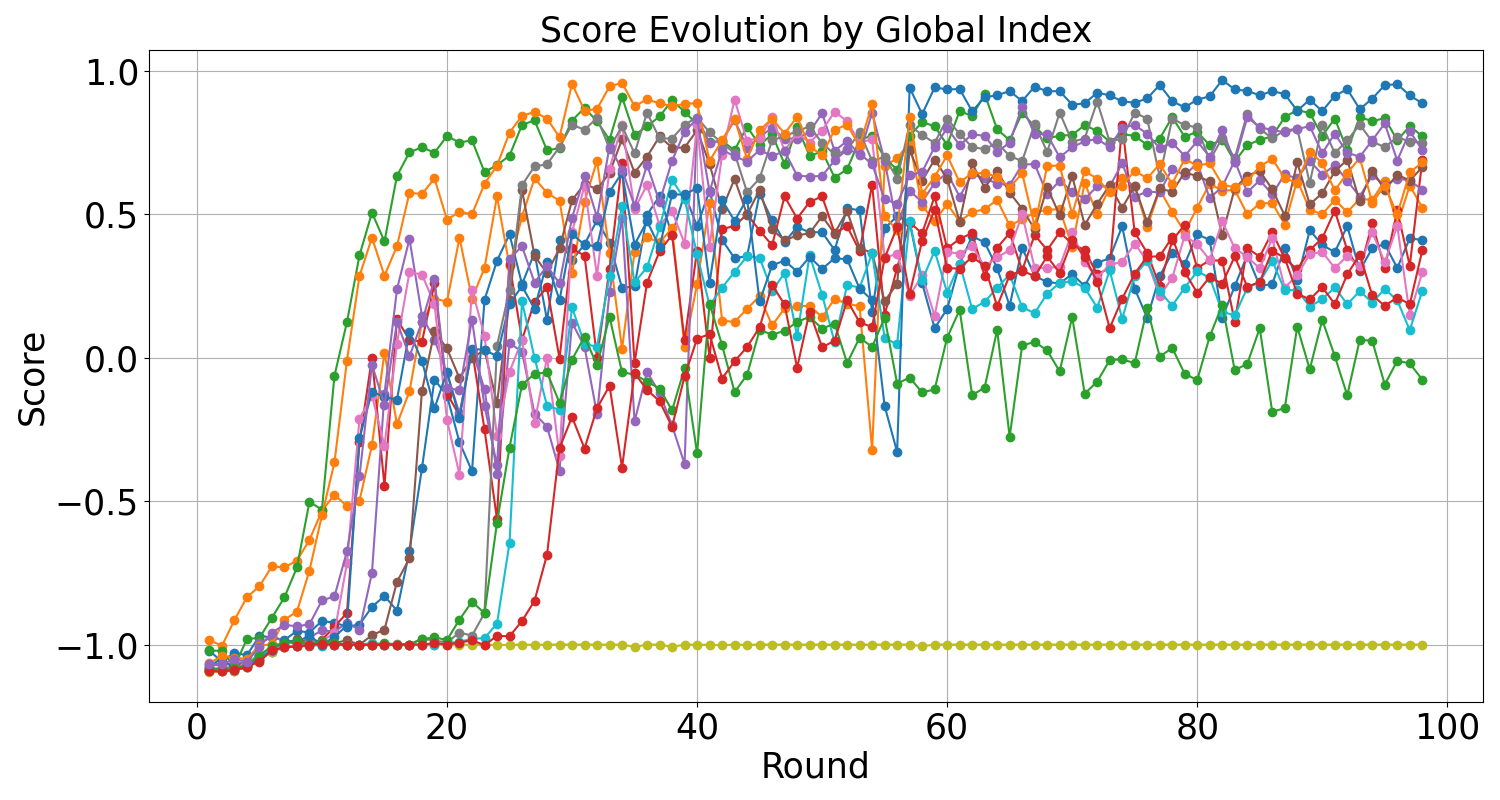
\includegraphics[width=\linewidth]{imgs/REINFORCE++.png}
\caption{REINFORCE++}
\end{subfigure}
\caption{Training traces on the small prompt set. The panels display within-run dynamics over 400 rounds for GRPO and 100 rounds for \ours.}
\label{fig:small_curves}
\end{figure}
